در این پوشه به بانک اطلاعات پرداخته می‌شود و تمام اطلاعات از پایگاه داده واکشی می‌شود.

\begin{figure}[H]
	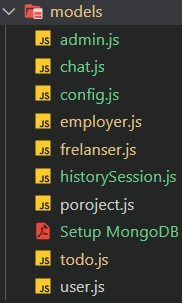
\includegraphics[width=.3\textwidth]{Folders-Files/models.png}
	\centering
	\caption{ساختار پوشه مدل}
	\label{fig:folder-models}
\end{figure}

\paragraph{فایل user}
در این فایل به بانک اطلاعات برای ثبت اطلاعات کاربر از جمله مشخصات شناسنامه‌ای، اطلاعات کاربری و رمز و ... پرداخته شده است.

\paragraph{فایل employer}
در این فایل به بانک اطلاعات برای اطلاعات داشبورد کارفرما مانند ثبت و بروزرسانی پروژه، دریافت پیشنهادهای انجام پروژه و ... پرداخته شده است.

\paragraph{فایل frelanser}
در این فایل به بانک اطلاعات برای ‌اطلاعات داشبورد فریلنسر مانند ثبت رزومه، ثبت پیشنهاد برای انجام پروژه و ... پرداخته شده است.
